\localauthor{Sebastian Vogt, Johannes Garstenauer, Johann Schicho}

Im Folgenden Kapitel wird für jedes Package der Autor dieses Abschnitts des Klassendiagramms genannt.

\newcommand{\classtable}[1]{\begin{longtable}[H]{m{5cm}m{9cm}}
                                \hline
                                \textbf{Klassenname} & \textbf{Beschreibung} \\
                                \hline
                                \hline
                                #1
\end{longtable}
}

\newcommand{\classentry}[2]{\textbf{#1} & #2 \\
}

\subsection{Klassendiagramm}

\localauthor{Sebastian Vogt}
Im folgenden Klassendiagramm wurden folgenden Konventionen verwendet:
\begin{itemize}
    \item Properties sind als private Attribute modelliert.
    Konstruktoren sind ausgespart.
    \item Referenzattribute auf andere Klassen des Diagramms sind als Pfeile dargestellt.
    Diese haben standardmäßig keine Getter und Setter, außer anders angegeben.
    \item Konstruktoren sind ausgespart, außer dieser ist privat.
    \item In den Backingbeans sind Attribute, die lediglich einen Anzeigetext aus einem Ressourcebundle laden, nicht angegeben.
\end{itemize}

\begin{figure}[H]
	\centering
	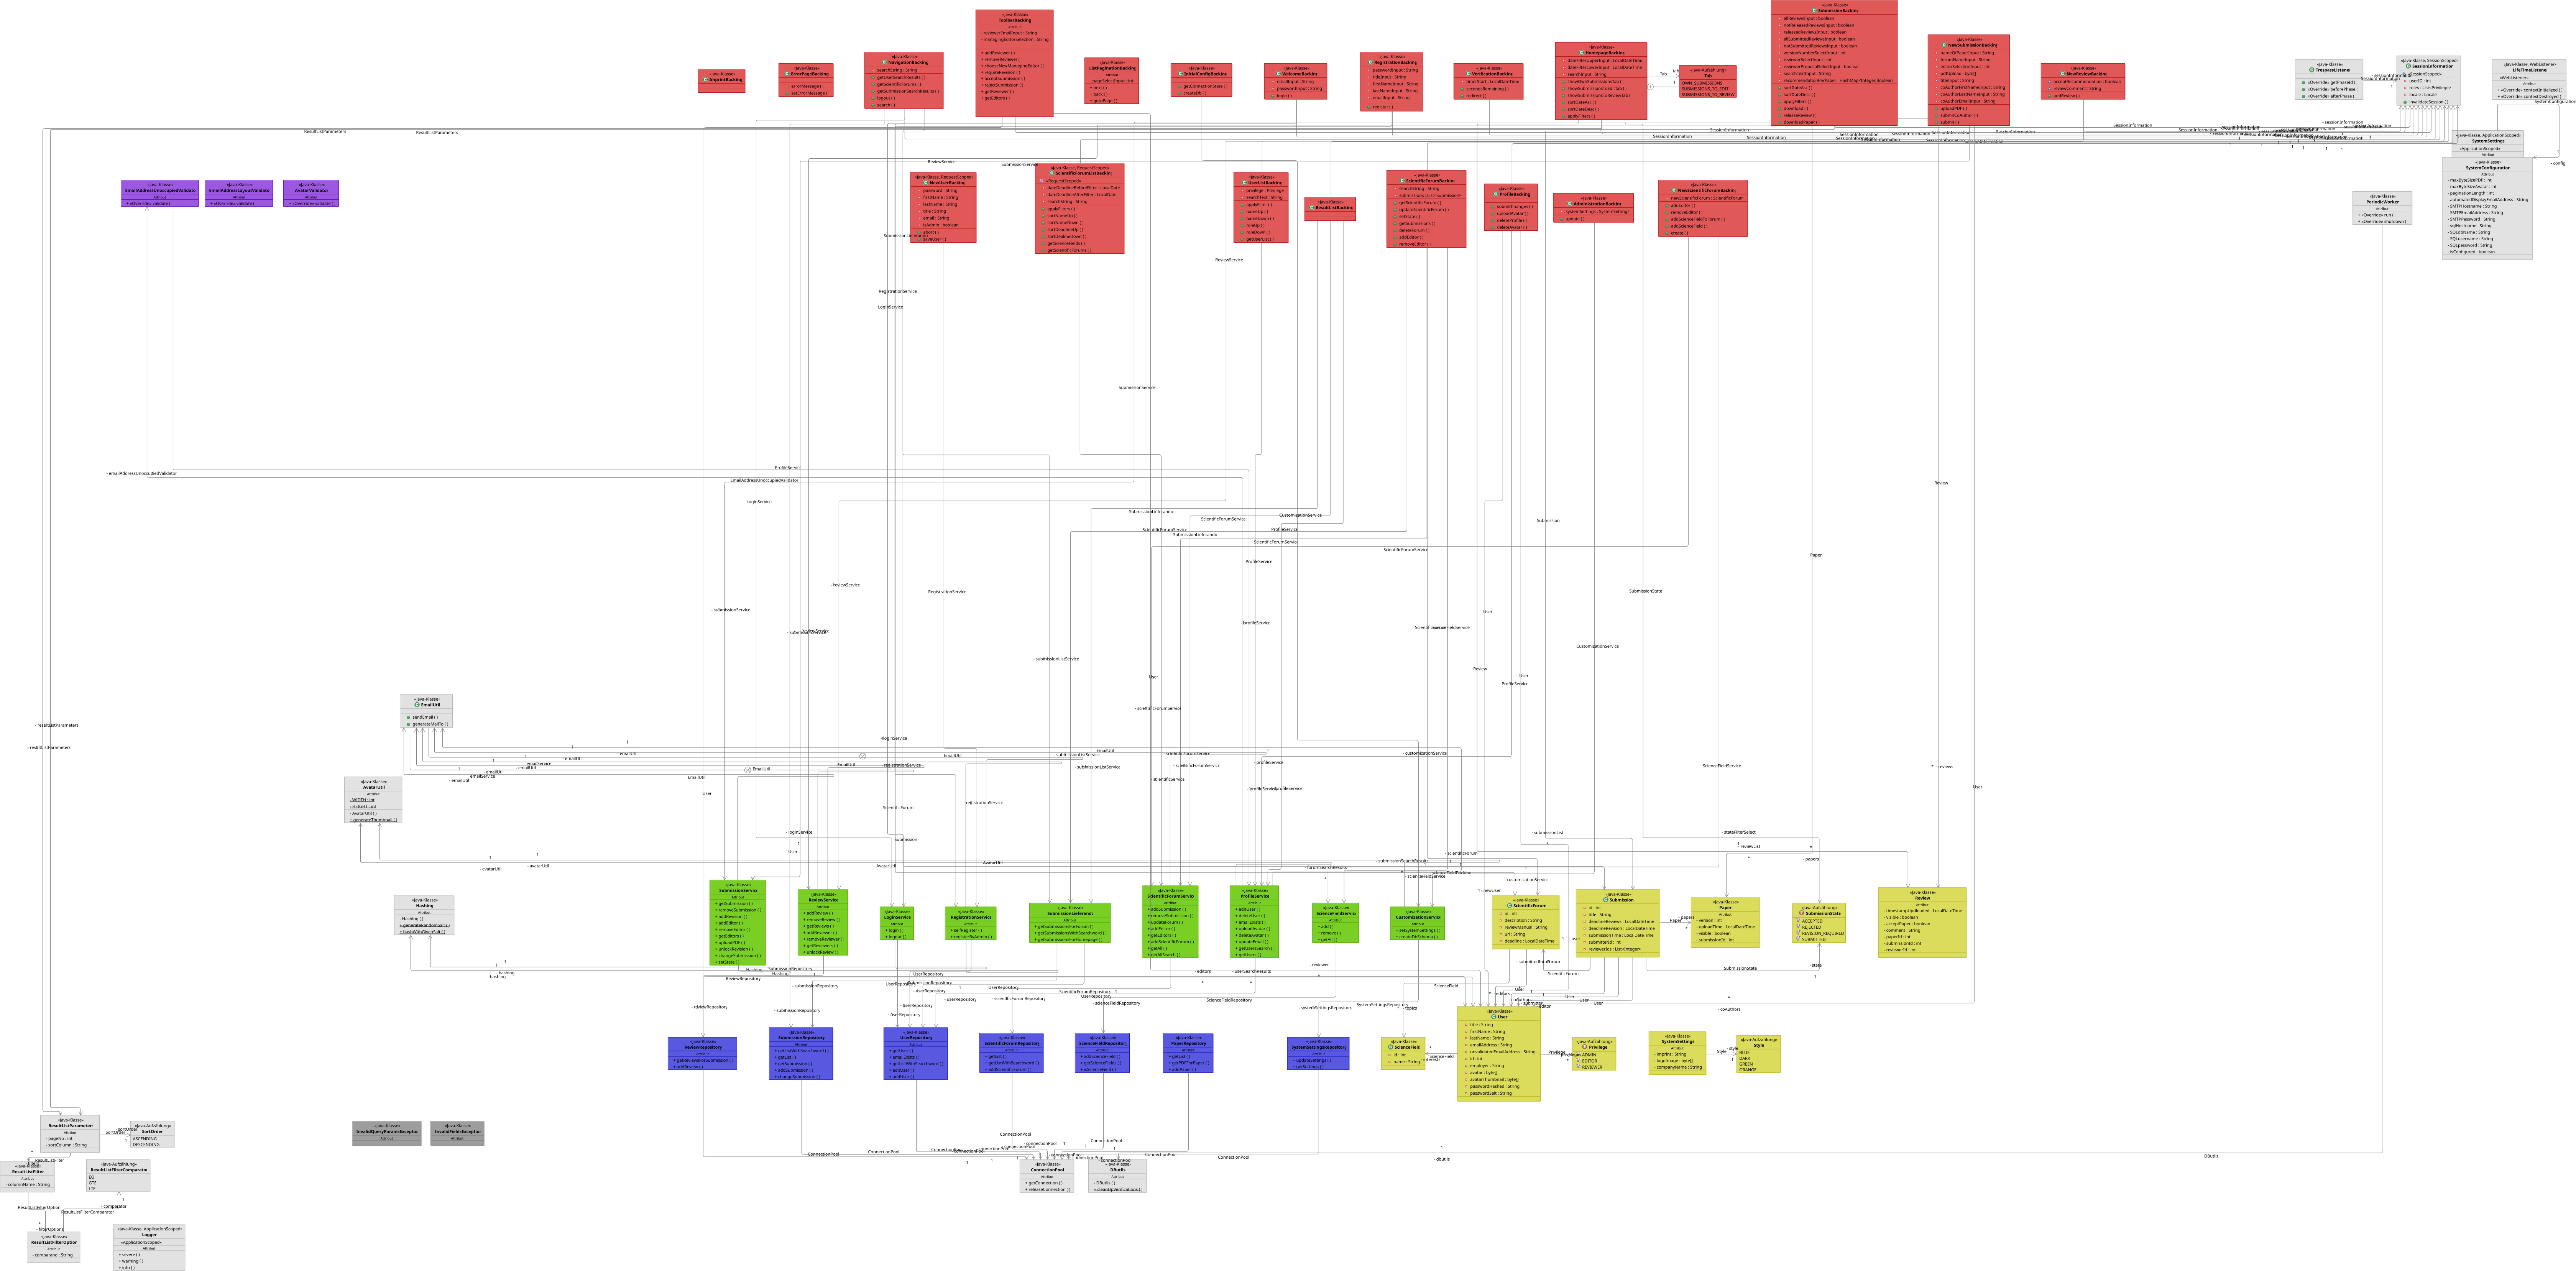
\includegraphics[width=\linewidth]{graphics/klassendiagramm_png}
\end{figure}

% Hier Klassendiagramm mal irgendwann einfügen.

\subsection{Klassenbeschreibungen}

\subsubsection{de.lases.business.service}

\localauthor{Johannes Garstenauer}

\begin{figure}[H]
	\centering
	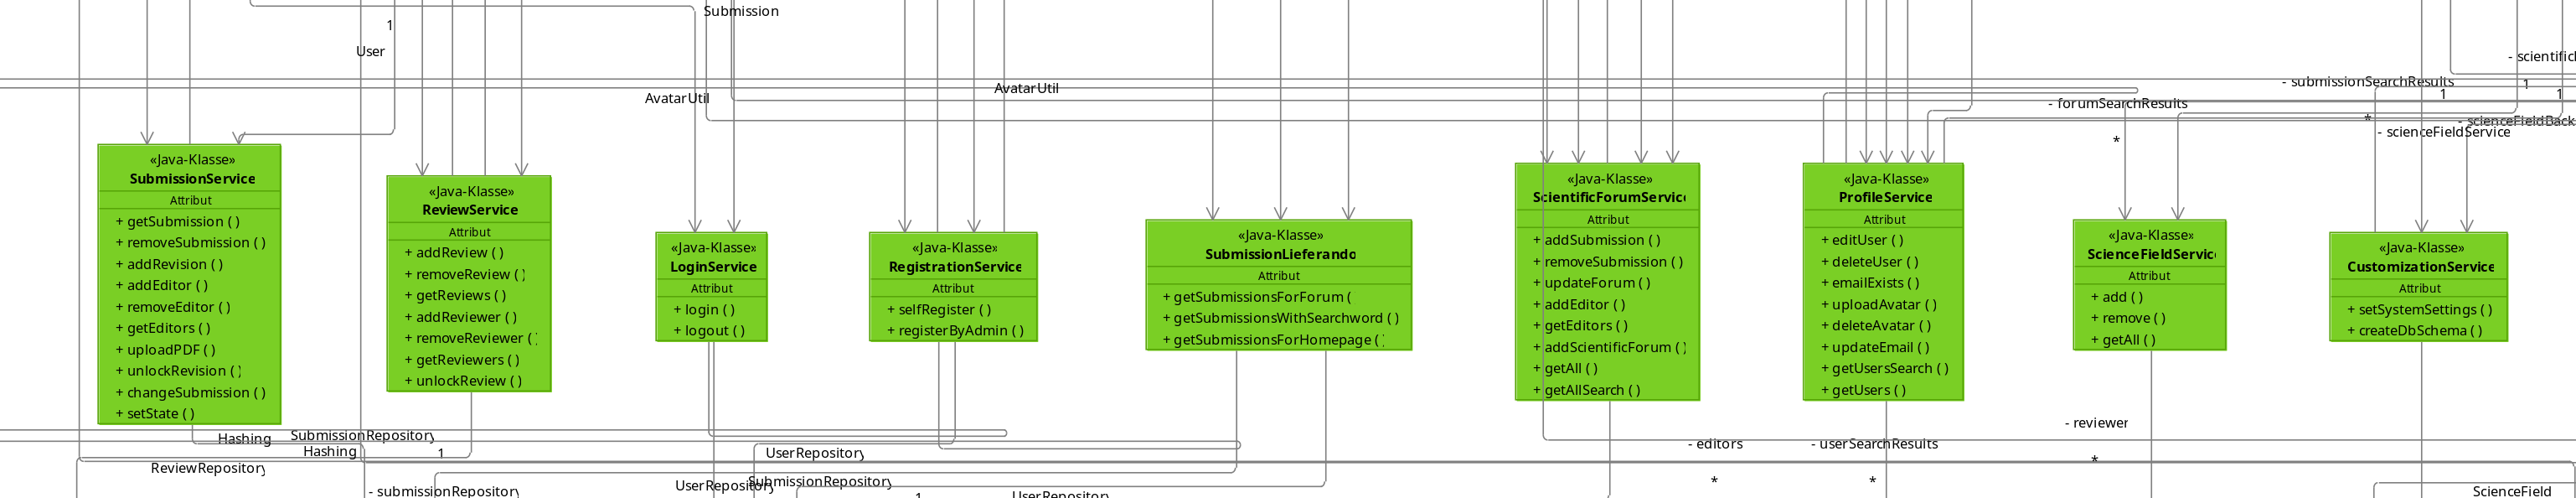
\includegraphics[width=0.9\linewidth]{graphics/business_service}
\end{figure}

\classtable{
	\classentry{CustomizationService}{Provides methods for the manipulation of system settings.}
	\classentry{ScienceFieldService}{Provides methods for adding and removing scientific categories.}
	\classentry{ProfileService}{Provides methods for the manipulation and removal of users.}
	\classentry{ScientificForumService}{Provides methods for the manipulation and creation of scientific forums.}
	\classentry{SubmissionLieferando}{Provides methods for delivering lists of submissions, taking into account
		their filtering, sorting and calling user.}
	\classentry{RegistrationService}{Provides methods for the creation of users.}
	\classentry{LoginService}{Provides methods for the login and logout operations.}
	\classentry{ReviewService}{Provides methods for the delivery, creation and removal of reviews.}
	\classentry{SubmissionService}{Provides methods for the delivery, creation, removal and manipulation of submissions.}
}

\subsubsection{de.lases.business.utils}

\localauthor{Johannes Garstenauer}

\begin{figure}[H]
	\centering
	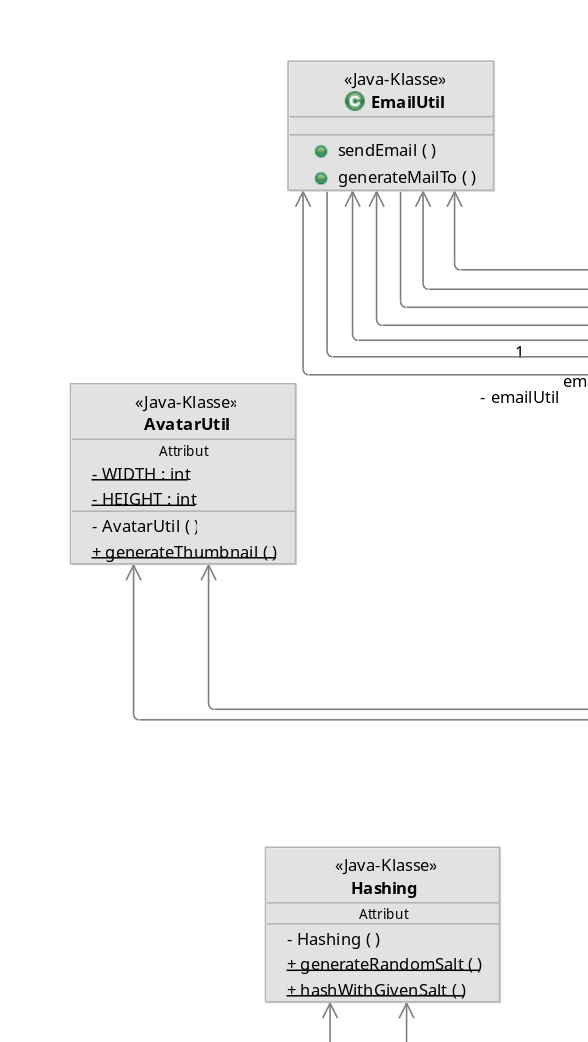
\includegraphics[height=3cm]{graphics/business_util}
\end{figure}

\classtable{
	\classentry{AvatarUtil}{Provides support in the generation of a thumbnail from an image.}
	\classentry{Hashing}{Provides support in the hashing of passwords.}
	\classentry{EmailUtil}{Provides support in the sending of emails and creation of mailto links.}
}

\subsubsection{de.lases.global.util}

\localauthor{Johann Schicho}

\begin{figure}[H]
	\centering
	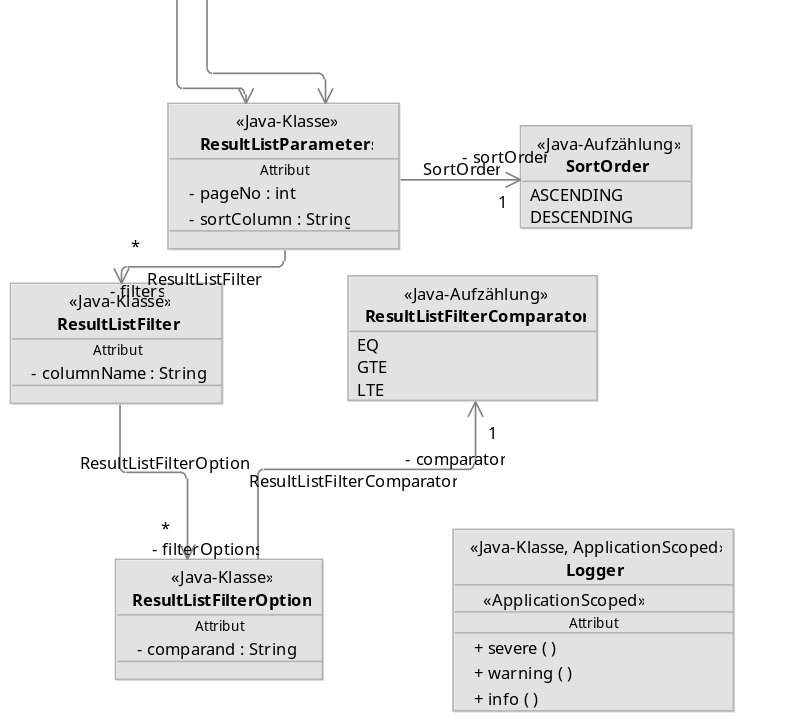
\includegraphics[height=3cm]{graphics/global_util}
\end{figure}

\classtable{
	\classentry{Logging}{This Logger allows logging in different log-levels.}
    \classentry{ResultListParameters}{This class bundles parameters for requesting lists from the database. This includes page numner, sorting of the results and filtering of the results}
    \classentry{SortOrder}{A List can be sorted in ascending or descending order}
    \classentry{ResultListFilter}{A filter that can be applied on a column of a table}
    \classentry{ResultListFilterOption}{A single comparison that can be used to construct a ResultListFilter}
    \classentry{ResultListFilterComparator}{The three comparators equal to, less than or equal and greater than or equal}
}

\subsubsection{de.lases.business.internal}

\localauthor{Johann Schicho}

\begin{figure}[H]
	\centering
	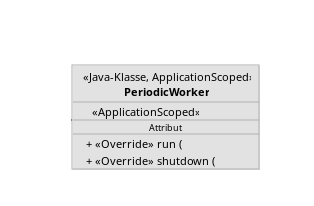
\includegraphics[height=3cm]{graphics/business_internal}
\end{figure}

\classtable{
	\classentry{TrespassListener}{Manages user access to resources, most importantly webpages.}
	\classentry{SessionInformation}{Wraps data saved in the session.}
	\classentry{LifeTimeListener}{Takes care of system start and shutdown operations}
	\classentry{PeriodicWorker}{Takes care of periodical database cleanup jobs.}
	\classentry{SystemSettings}{Loads and updates the systems' configuration.}
	\classentry{SystemConfiguration}{Wraps data used for the system configuration.}
}

\subsubsection{de.lasses.control.validation}

\localauthor{Sebastian Vogt, ff.}

\begin{figure}[H]
	\centering
	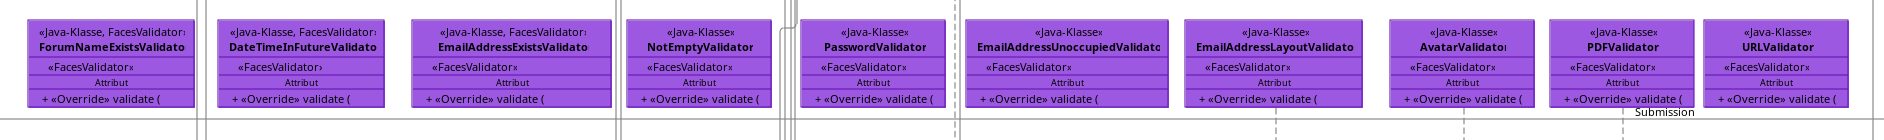
\includegraphics[height=3cm]{graphics/control_validation}
\end{figure}

\classtable{
    \classentry{AvatarValidation}{Validates that a suitable avatar image has been uploaded.}
\classentry{EmailAddressLayoutValidation}{Validates that the email regex pattern is ok.}
\classentry{EmailAdressUnoccupiedValidator}{Validates that a given email is not already in use within the system.}
}

\subsubsection{de.lases.global.transport}

\begin{figure}[H]
	\centering
	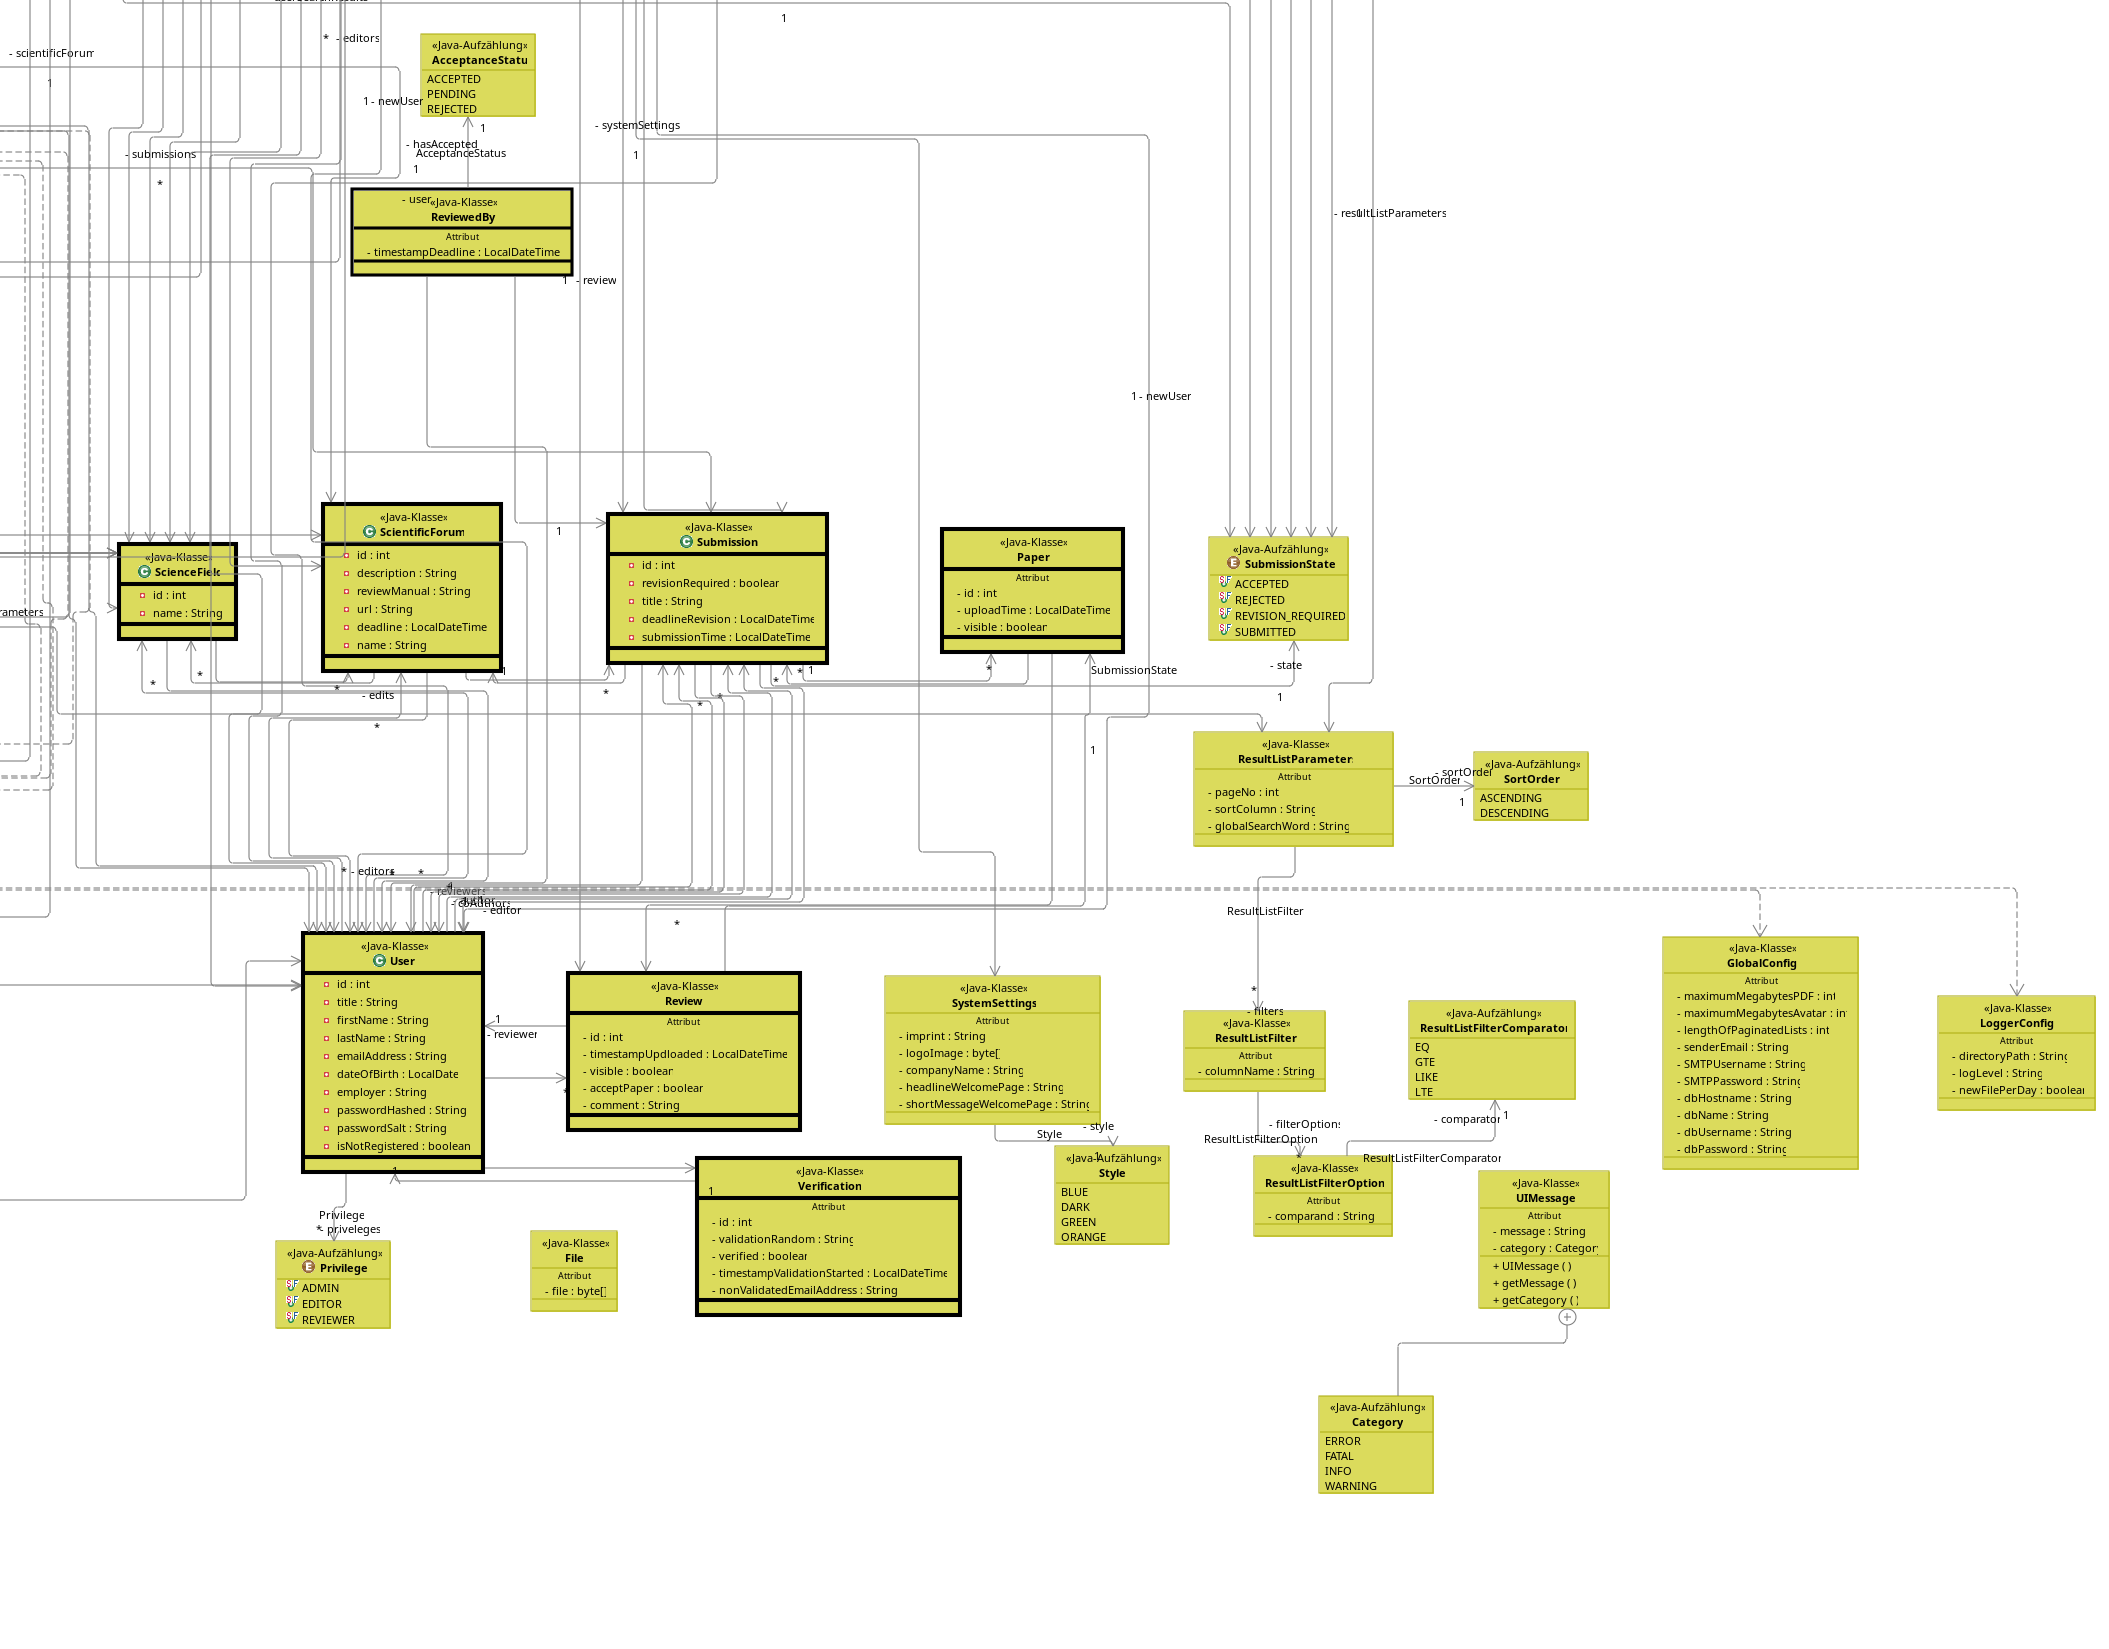
\includegraphics[height=3cm]{graphics/global_transport}
\end{figure}

\classtable{
    \classentry{Paper}{This DTO represents a paper.}
    \classentry{Privilege}{This represents a user privilege.}
    \classentry{Review}{This DTO represents a review.}
    \classentry{ScienceField}{This DTO represents a field of Science.}
    \classentry{ScientificForum}{This DTO represents a forum}
    \classentry{Style}{This represents a user interface style.}
    \classentry{Submission}{This DTO represents a submission.}
    \classentry{SubmissionState}{This represents a submissions state.}
    \classentry{SystemSettings}{This DTO represents the system settings.}
    \classentry{User}{This DTO represents a user.}
}

\subsubsection{de.lases.persistence.repository}

\begin{figure}[H]
	\centering
	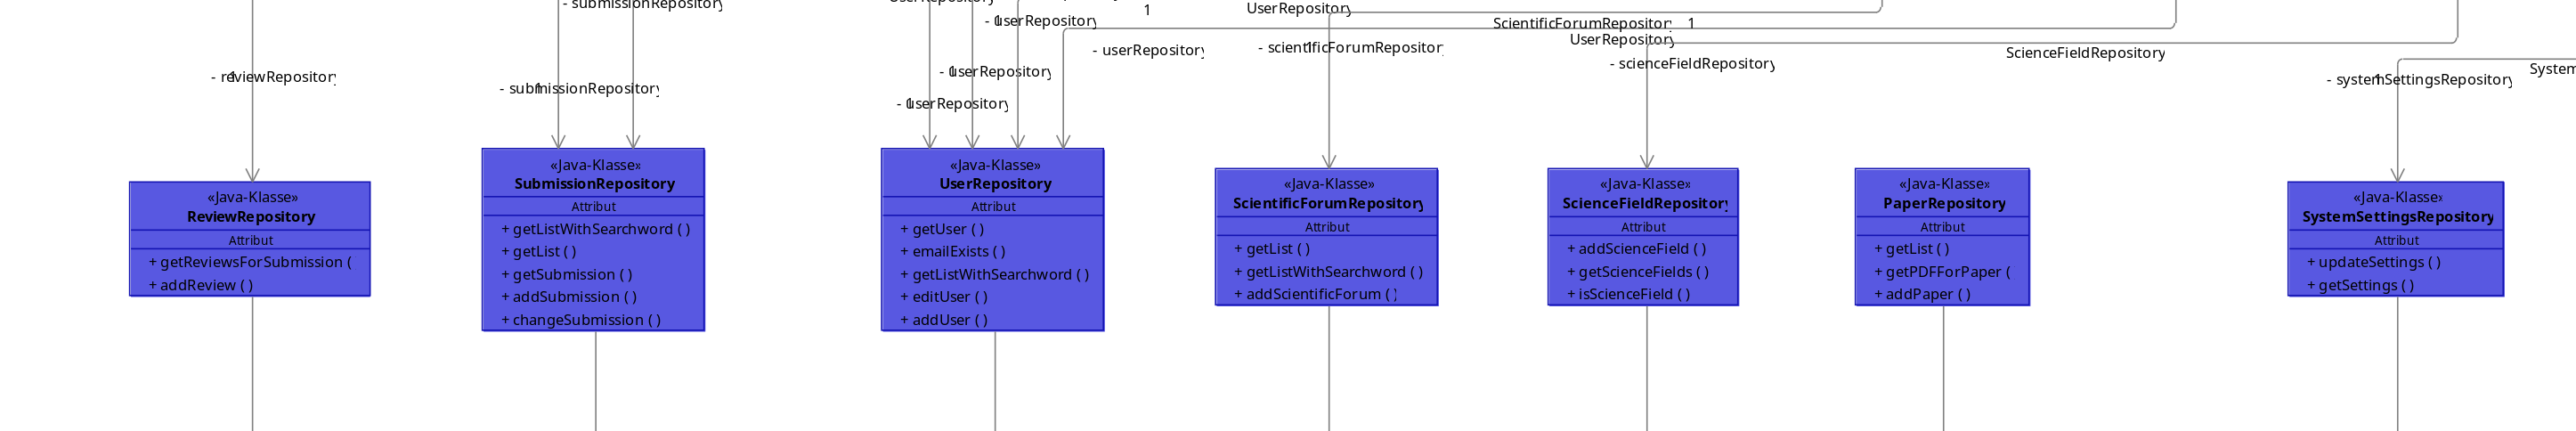
\includegraphics[width=0.9\linewidth]{graphics/persistence_repository}
\end{figure}

\classtable{
    \classentry{PaperRepository}{This repository can get the list of papers for a submission or add new ones.}

    \classentry{ReviewRepository}{This repository can get the reviews for a certain submission and add new ones.}

    \classentry{ScienceFieldRepository}{This repository can get or add new fields of science from/to the database.}

    \classentry{ScientificForumRepository}{This repository can get a list of journals and conferences or add new ones.}

    \classentry{SubmissionRepository}{This repository allows CRUD operations on submissions.}

    \classentry{SystemSettingsRepository}{This repository can read or update the system settings.}

    \classentry{UserRepository}{This repository allows CRUD operations on users.}
}

\subsubsection{de.lases.persistence.util}

\begin{figure}[H]
	\centering
	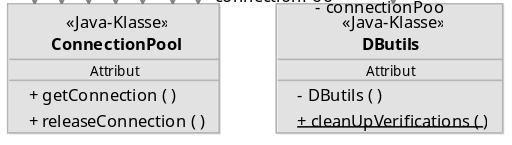
\includegraphics[height=2cm]{graphics/persistence_util}
\end{figure}

\classtable{
    \classentry{ConnectionPool}{Provides and manages connections to the database.}
}

\subsubsection{de.lases.persistence.exception}

\begin{figure}[H]
	\centering
	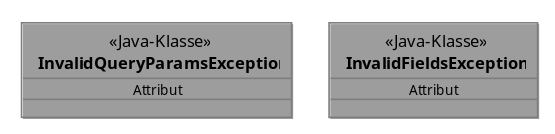
\includegraphics[height=2cm]{graphics/persistence_exception}
\end{figure}

\classtable{
    \classentry{InvalidFieldsException}{Hints at an invalid field in a dto.}
    \classentry{InvalidQueryParamsException}{Hints at invalid filter or sort parameters given to the query.}
}

\subsubsection{de.lases.control.backing}

\begin{figure}[H]
	\centering
	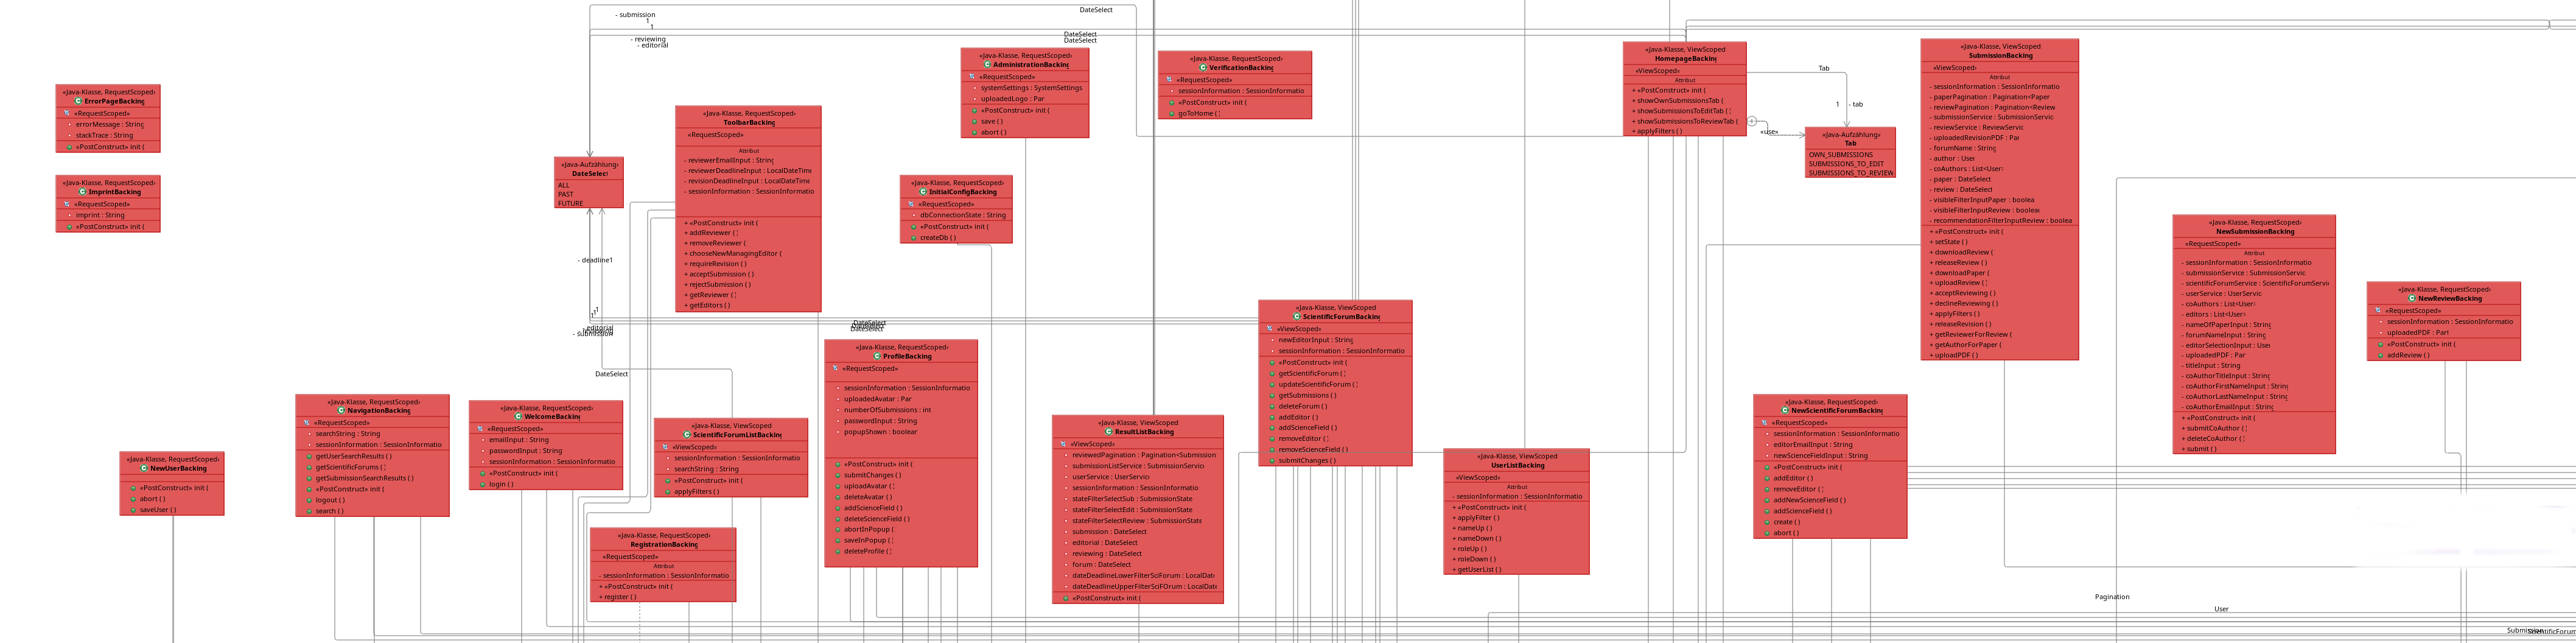
\includegraphics[width=0.9\linewidth]{graphics/control_backing}
\end{figure}

\classtable{
	\classentry{NewSubmissionBacking}{Backing bean for the page for creating a new submission.}
    \classentry{SubmissionBacking}{Backing bean for the submission page.}
    \classentry{NewReviewBacking}{Backing bean for the page for creating adding a new review.}
    \classentry{VerificationBacking}{Backing bean for the verification page.}
    \classentry{ToolbarBacking}{Backing bean for the side toolbar.}
    \classentry{NavigationBacking}{Backing bean for the navigation bar.}
    \classentry{WelcomeBacking}{Backing bean for the welcome and login page.}
    \classentry{RegistrationBacking}{Backing bean for the registration page.}
    \classentry{HomepageBacking}{Backing bean for the homepage for logged in users.}
    \classentry{NewUser}{Backing bean for the page for adding a new user.}
    \classentry{ScientificForumListBacking}{Backing bean for the list of scientific forums.}
    \classentry{UserListBacking}{Backing bean for the list of users.}
    \classentry{ResultListBacking}{Backing bean for the search result page.}
    \classentry{ScientificForumBacking}{Backing bean for the scientific forum page.}
    \classentry{NewScientificForumBacking}{Backing bean for the page for adding a new forum.}
    \classentry{ProfileBacking}{Backing bean for the profile page.}
    \classentry{AdministrationBacking}{Backing bean for the administration page.}
}

